% ================================================================
% The Retrieve and Connect version of latex/starters/targeted/KS3/algebra/expandingBracketsStarter.tex
%
% This is the same deck as the one above, made by renaming the titles in it.
% Every slide that was a numbered starter is now titled
% "Retrieve and Connect", and the word is renamed wherever else a title
% used it. Nothing outside a title has been changed.
%
%   made from           latex/starters/targeted/KS3/algebra/expandingBracketsStarter.tex
%   retitling rules     version 1
%
% Please don't edit this file. It is written again from the one it was
% made from whenever that changes, so an edit here would be lost - edit
% that file instead and this one follows.
% ================================================================
\documentclass{beamer}

% Theme (optional but nice)
\usetheme{Madrid}

% Maths
\usepackage{amsmath}

% Graphics
\usepackage{tikz}

% ================================================================
% Answer-overlay helpers
% ================================================================
\newcommand{\ablank}[1]{%
  \alt<2>{\textcolor{red}{#1}}{\underline{\phantom{#1}}}%
}
\newcommand{\ashow}[1]{\uncover<2->{\textcolor{red}{\small #1}}}
\newcommand{\ashowq}[1]{\alt<2->{\textcolor{red}{\small #1}}{?}}

% Answers drawn straight on to a TikZ diagram, revealed on overlay 2 like \ashow.
% Space is reserved on overlay 1, so the diagram does not move between slides.
\usetikzlibrary{overlay-beamer-styles}
\tikzset{
  ans/.style     = {red, thick, visible on=<2->},
  ansfill/.style = {red!15, visible on=<2->},
  anslab/.style  = {red, font=\tiny, visible on=<2->},
}

\begin{document}

% ---------- STARTER (PRIOR KNOWLEDGE) ----------
\begin{frame}{Retrieve and Connect: Prior Knowledge}
\begin{minipage}[t]{0.48\textwidth}

\begin{block}{1) Arithmetic}
\Large
\[
13 + 9 = \ablank{22}
\]
\end{block}

\vspace{6.2em}

\begin{block}{3) Collect like terms}
\Large
\[
3b + 4 + 2b = \ablank{5b+4}
\]
\end{block}

\end{minipage}\hfill
\begin{minipage}[t]{0.48\textwidth}

\begin{block}{2) Box Method}
\centering
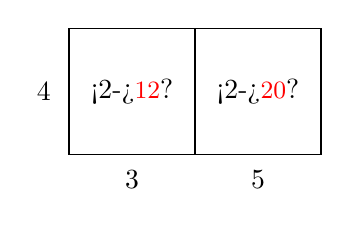
\begin{tikzpicture}[scale=0.8]

\draw (0,0) rectangle (4,2);
\draw (2,0) -- (2,2);

\node at (1,-0.4) {$3$};
\node at (3,-0.4) {$5$};
\node at (-0.4,1) {$4$};

\node at (1,1) {\ashowq{12}};
\node at (3,1) {\ashowq{20}};

\end{tikzpicture}

\vspace{0.4em}
Find the total area. \ashow{Total area $= 32$}

\end{block}

\vspace{0.6em}

\begin{block}{4) Expand the bracket}
\Large
\[
2(x+6) = \ablank{2x+12}
\]
\end{block}

\end{minipage}
\end{frame}


% ---------- STARTER ANSWERS ----------
\begin{frame}{Retrieve and Connect: Answers}
\begin{minipage}[t]{0.48\textwidth}

\begin{block}{1) Arithmetic}
\Large
\[
13 + 9 = \textcolor{red}{22}
\]
\end{block}

\vspace{6.2em}

\begin{block}{3) Collect like terms}
\Large
\[
3b + 4 + 2b = \textcolor{red}{5b + 4}
\]
\end{block}

\end{minipage}\hfill
\begin{minipage}[t]{0.48\textwidth}

\begin{block}{2) Box Method}
\centering
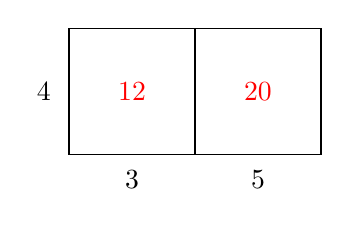
\begin{tikzpicture}[scale=0.8]

\draw (0,0) rectangle (4,2);
\draw (2,0) -- (2,2);

\node at (1,-0.4) {$3$};
\node at (3,-0.4) {$5$};
\node at (-0.4,1) {$4$};

\node at (1,1) {\textcolor{red}{12}};
\node at (3,1) {\textcolor{red}{20}};

\end{tikzpicture}

\vspace{0.4em}
\textcolor{red}{Total area = 32}

\end{block}

\vspace{0.6em}

\begin{block}{4) Expand the bracket}
\Large
\[
2(x+6) = \textcolor{red}{2x + 12}
\]
\end{block}

\end{minipage}
\end{frame}


\end{document}